% !TeX encoding = UTF-8
% !TeX spellcheck = pl_PL

\def\filename{rozdzial4}
\chapter{Metodyka badania}

\section{Model sieci neuronowej}

\subsubsection{Wstęp}
Badania przeprowadzono w środowisku Python z wykorzystaniem interaktywnego notatnika Jupyter Notebook.
Obliczenia wykonywano na komputerze wyposażonym w kartę graficzną NVIDIA GeForce RTX 5070 Ti, wspierającą akcelerację obliczeń w oparciu o technologię CUDA. 
Wykorzystanie GPU pozwoliło znacząco skrócić czas trenowania modeli konwolucyjnych oraz umożliwiło przeprowadzenie złożonych eksperymentów w rozsądnym czasie obliczeniowym.
	
Podczas konfiguracji i trenowania sieci neuronowych zastosowano zestaw bibliotek wspierających przetwarzanie danych, budowę modeli głębokiego uczenia oraz analizę wyników. 
Główne pakiety wykorzystane w badaniu to:
\begin{itemize}
	\item \textbf{pandas} - narzędzie do analizy danych tabelarycznych, umożliwiające ich wczytywanie, filtrowanie oraz łączenie metadanych z obrazami \cite{pandas},
	\item \textbf{numpy} - biblioteka numeryczna wykorzystywana do operacji na macierzach, wektorach oraz konwersji obrazów do formatów wejściowych modeli \cite{Harris_2020},
	\item \textbf{matplotlib} oraz \textbf{seaborn} – pakiety do wizualizacji danych, używane do generowania wykresów, prezentacji obrazów oraz analizy rozkładów klas \cite{matplotlib, seaborn},
	\item \textbf{tensorflow} oraz \textbf{keras} - pakiety głębokiego uczenia wykorzystywane do trenowania modeli konwolucyjnych oraz obsługi akceleracji GPU \cite{abadi2016tensorflowlargescalemachinelearning},
	\item \textbf{torch} oraz \textbf{torchvision} - biblioteki do budowy i trenowania sieci neuronowych, wykorzystywane do transformacji obrazów, przygotowania zbiorów danych oraz korzystania z gotowych architektur modeli \cite{1874254, paszke2019pytorchimperativestylehighperformance},
	\item \textbf{scikit-learn} - zestaw narzędzi do analizy predykcyjnej, umożliwiający podział danych na zbiory treningowe i testowe, obliczanie wag klas oraz ewaluację modeli \cite{pedregosa2018scikitlearnmachinelearningpython},
	\item \textbf{Pillow (PIL)} - biblioteka służąca do podstawowego przetwarzania obrazów, w tym ich wczytywania, skalowania i konwersji.
\end{itemize}

\subsection{Obróbka danych}
Zbiory danych HAM10000, PAD‑UFES‑20, derm7pt, ISIC 2020 oraz BCN20000 pobrano lokalnie i załadowano z dysku.
Każdy zbiór składał się z archiwum ZIP zawierającego obrazy oraz pliku CSV z metadanymi opisującymi przypadki kliniczne. 
W pierwszym etapie rozpakowano wszystkie archiwa, a następnie dla każdego zbioru utworzono kolumnę path, która wskazywała pełną ścieżkę do konkretnego pliku graficznego. 
Umożliwiło to późniejsze elastyczne operowanie na obrazach oraz ich łączenie w jeden zbiór.
	
\begin{lstlisting}[language=Python, caption=Funkcja do rozpakowywania archiwów ZIP]
def unzip(zip_path, extract_to):
	if not os.path.exists(zip_path):
		print(f"ZIP nie istnieje: {zip_path}")
		return
	os.makedirs(extract_to, exist_ok=True)
	with zipfile.ZipFile(zip_path, 'r') as zip_ref:
		zip_ref.extractall(extract_to)
\end{lstlisting}

Po rozpakowaniu zdjęć przypisano każdemu rekordowi dokładnej lokalizacji odpowiadającego mu obrazu na dysku.
Każdy zbiór wymagał indywidualnego podejścia, ponieważ różniły się one strukturą katalogów oraz sposobem nazewnictwa plików.
Następnie przeprowadzono weryfikację integralności danych polegającą na próbie otwarcia każdego pliku graficznego.
Obrazy, które generowały wyjątek, zostały usunięte ze zbioru, co zapewniło poprawność danych wejściowych wykorzystywanych w dalszych etapach analizy.

\begin{lstlisting}[language=Python, caption=Funkcja do usuwania uszkodzonych obrazów]
def remove_corrupted(metadata, path_column="path"):
	good, bad = [], []
	for path in metadata[path_column]:
		try:
			if path is None or not os.path.exists(path):
				bad.append(path)
				continue
			img = Image.open(path)
			img.verify()
			good.append(path)
		except Exception:
			bad.append(path)
	return metadata[metadata[path_column].isin(good)].reset_index(drop=True)
\end{lstlisting}

Wszystkie zbiory obejmowały łącznie 42 klasy diagnostyczne, jednak ich nazwy znacząco różniły się między zbiorami.
W celu uproszczenia i ujednolicenia zbiorów zdecydowano się na zredukowanie klas do siedmiu kategorii zmian skórnych, które szczegółowo opisano w Rozdziale 3 i przedstawiono w tabeli \ref{tab:klasy_ujednolicone}.
Ujednolicenie pozwoliło na spójne etykietowanie danych pochodzących z różnych źródeł.
	
Ze względu na silną nierównowagę klas przeprowadzono zastosowano oversampling, czyli technikę polegającą na sztucznym zwiększeniu liczby przykładów klas rzadkich poprzez wielokrotne powielanie.
W efekcie liczebność każdej kategorii została zwiększona do 5000 przykładów, co odpowiadało 14,3\% całego zbioru.
Rozkład klas przed i po oversamplingu przedstawiono odpowiednio na wykresach \ref{fig:classes_bar}, \ref{fig:classes_pie} oraz \ref{fig:oversampling_classes} w Rozdziale 3.

\begin{figure}[h!]
	\centering
	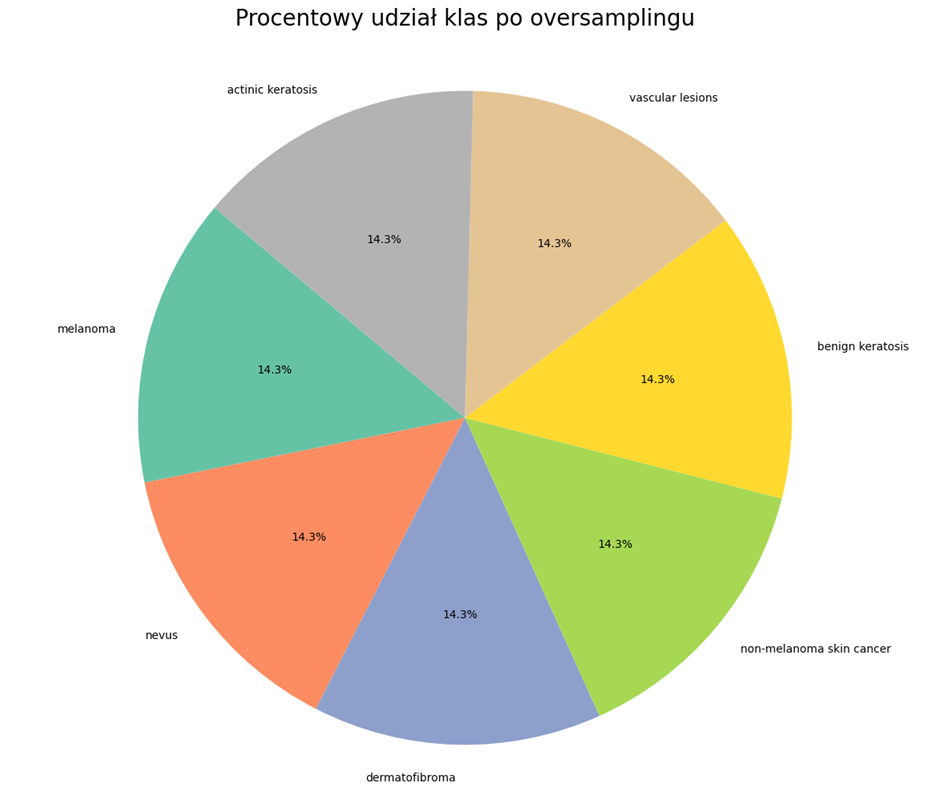
\includegraphics[width=0.9\linewidth]{oversampling_classes}
	\caption{Rozkład klas po oversamplingu}
	\source{Opracowanie własne}
	\label{fig:oversampling_classes}
\end{figure}

\subsubsection{Przygotowanie do trenowania}
Po oczyszczeniu i ujednoliceniu danych zbiór podzielono na dwa główne podzbiory, jeden obejmujący zdjęcia dermoskopowe a drugi, znacznie mniejszy, obrazy wykonane aparatem telefonu.

Następnie dokonano podziału danych dermoskopowych na zbiór testowy, który stanowił 20\% danych.
Z pozostałych danych 10\% przeznaczono na zbiór walidacyjny i 90\% na zbiór treningowy.

Zbiór obejmujący dane zdjęć wykonanych aparatem telefonu podzielono na zbiór treningowy i walidacyjny w proporcji 80 do 20.

W kolejnym kroku połączono oba zbiory treningowe w jeden, aby model mógł uczyć się jednocześnie zdjęć dermoskopowych jak i telefonicznych.

Ostateczne proporcje zbiorów wynosiły
\begin{itemize}
	\item dane treningowe - x przykładów
	\item dane walidacyjne - x przykładów obrazów dermoskopowych, x przykładów obrazów telefonicznych
	\item dane testowe - x przykładów
\end{itemize}

Wyznaczenie dwóch zbiorów walidacyjnych umożliwia ocenę zdolności modelu do generalizacji na dwóch różnych typach obrazów, co jest kluczowe w kontekście zastosowań klinicznych.

Do przygotowania danych do trenowania wykorzystano klasę ImageDataGenerator z biblioteki Keras, która umożliwia wykonywanie losowych transformacji obrazów podczas trenowania, które zwiększają różnorodność danych treningowych.
Zastosowano losowy obrót w zakresie 10 stopni, przybliżenie do 10\% oraz odbicie obrazu w płaszczyźnie poziomej.
Augmentacja pomaga ograniczyć przeuczenie (ang. \textit{overfitting}) i lepiej odzwierciedla zmienność jakości zdjęć wykonywanych telefonem.

Dla zbiorów walidacyjnych i testowych zastosowano generatory bez augmentacji aby zapewnić obiektywną ocenę modelu.

\begin{lstlisting}[language=Python, caption=Definicja ImageDataGeneratora dla klasy treningowej]
train_datagen = ImageDataGenerator(
	preprocessing_function=preprocess_input,
	rotation_range=10,
	zoom_range=0.1,
	horizontal_flip=True,
	fill_mode='nearest'
)
\end{lstlisting}

Następnie utworzono generatory wczytujące obrazy z dysku, skalujące je do rozmiaru 224 na 224 pikseli, kodujące etykiety oraz stosujące zdefiniowane transformacje.

W celu porównania skuteczności rożnych architektur konwolucyjnych sieci neuronowych zdefiniowano słownik modeli dostępnych w ramach biblioteki Keras.
Modele różnią się pod względem liczby parametrów, głębokości architektury oraz przeznaczenia.
Część z wybranych sieci, na przykład MobileNetV2 lub NASNetMobile zostało zaprojektowanych specjalnie z myślą o urządzeniach mobilnych, co jest istotne w kontekście implementacji systemu wykonującego inferencję na smartfonie.

\begin{lstlisting}[language=Python, caption=Słownik sieci neuronowych]
MODELS = {
	"MobileNetV2": tf.keras.applications.MobileNetV2,
	"VGG16": tf.keras.applications.VGG16,
	"NASNetMobile": tf.keras.applications.NASNetMobile,
	"ResNet50": tf.keras.applications.ResNet50,
	"InceptionV3": tf.keras.applications.InceptionV3,
	"EfficientNetB0": tf.keras.applications.EfficientNetB0,
	"DenseNet121": tf.keras.applications.DenseNet121,
}
\end{lstlisting}

\subsubsection{Przygotowanie do trenowania}
Aby umożliwić elastyczne trenowanie wielu modeli, stworzono wysokopoziomowy moduł TransferLearningTuner, który kompleksowo obsługuje cały proces trenowania z wykorzystaniem techniki transfer learning.
Konstruktor klasy przyjmuje między innymi nazwę modelu bazowego zdefiniowaną w słowniku, liczbę klas, generatory danych oraz parametry trenowania.

TransferLearningTuner w pierwszym kroku tworzy architekturę wczytując model bazowy i zamrażając jego wagi, co zapobiega degradacji wcześniej wyuczonych reprezentacji.
W kolejnym kroku dodano warstwy klasyfikacyjne, które redukują wymiar cech, stabilizują trenowanie oraz zapobiegają przeuczeniu.

Pierwszy etap trenowania polega na uczeniu wyłącznie warstw klasyfikacyjnych przy zamrożonych wagach modelu bazowego.
Domyślnie trenowanie w tym etapie składa się z pięciu epok i jest wykonywane z learning rate na poziomie 5e-5.
Do trenowania wykorzystano optymalizator Adam oraz funkcję straty CategoricalFocalCrossentropy, która redukuje wpływ klas dominujących na predykcje modelu.
Zdefiniowano również kilka funkcji wywoływanych po każdej epoce lub po zakończeniu procesu, polegających na zapisie najlepszych wag modelu, zatrzymanie trenowania po 3 epokach bez poprawy, redukcji learning rate przy stagnacji oraz minitorowanie różnic między domeną dermoskopową a zdjęć telefonicznych.

Drugi etap trenowania odmraża większość warstw modelu bazowego z wyjątkiem warstw BatchNormalization, które przechowują statystyki domenowe i ich trenowanie mogłoby destabilizować proces.
Odmrożenie warstw pozwala dostosować głębsze reprezentacje do specyfiki danych dermatologicznych.

Po zakończeniu trenowania wykonywana jest ewaluacja na zbiorze testowym a następnie generowana jest macierz pomyłek, wynik F1 dla każdej klasy oraz wykresy strat i dokładności.
Następnie wytrenowany model jest konwertowany do formatu TensorFlow Lite, umożliwiając wykorzystanie go do bezpośredniej inferencji na urządzeniu mobilnym.
Cały pipeline uruchamiany jest motodą run, która wykonuje oba etapy trenowania oraz pełną ewaluację.

\section{Aplikacja mobilna}
W ramach systemu zaprojektowano aplikację mobilną korzystającą z wybranego modelu.
Zdecydowano się na zaimplementowanie aplikacji na systemy Android z wykorzystaniem języka programistycznego Kotlin.
Do stworzenia elementów interfejsu graficznego użyto biblioteki Jetpack Compose.
Sieć neuronową uwzględniono w zasobach aplikacji i obsłużono za pomocą biblioteki TensorFlow Lite.

\begin{figure}[h!]
	\centering
	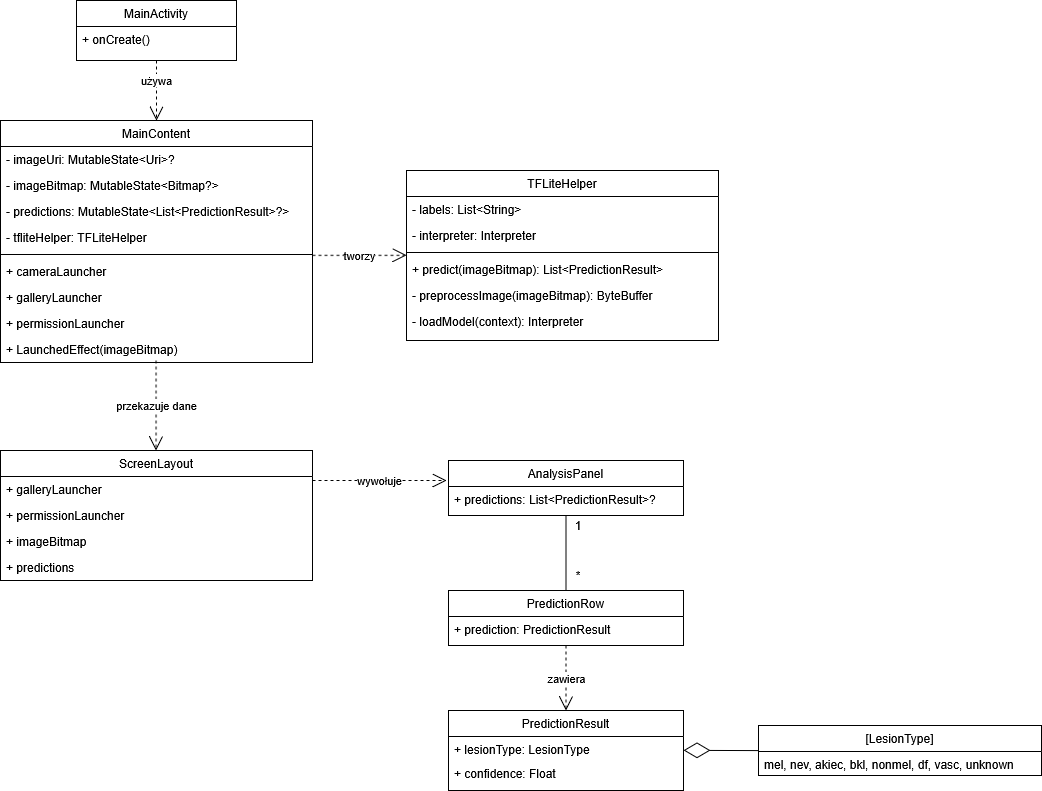
\includegraphics[width=0.9\linewidth]{diagram_klas}
	\caption{Diagram klas przedstawiający działanie aplikacji}
	\source{Opracowanie własne}
	\label{fig:diagram_klas}
\end{figure}

Diagram \ref{fig:diagram_klas} przedstawia pełną architekturę aplikacji, w której warstwa interfejsu użytkownika jest ściśle oddzielona od logiki przetwarzania obrazu i inferencji modelu uczenia maszynowego.
Klasa MainActivity pełni rolę punktu wejścia aplikacji i inicjuje środowisko Compose, delegując dalsze zarządzanie stanem i logiką do komponentu MainContent.
MainContent stanowi centralny element warstwy interfejsu użytkownika - przechowuje stan bieżącego obrazu, wyniki klasyfikacji oraz instancję klasy TFLiteHelper.
TFLiteHelper odpowiada za przygotowanie danych wejściowych, uruchomienie modelu TensorFlow Lite oraz przetworzenie wyników inferencji.
Obraz dostarczony przez użytkownika jest skalowany, normalizowany i konwertowany do formatu akceptowanego przez Interpreter z biblioteki TensorFlow Lite.
Następnie model zwraca wektor prawdopodobieństw, który jest mapowany na typy zmian skórnych zdefiniowane w enumeracji LesionType.
Każdy wynik jest reprezentowany jako obiekt PredictionResult, zawierający LesionType jak i poziom prawdopodobieństwa przynależności do danej grupy.
Stworzenie dedykowanej klasy umożliwia łatwą prezentacje wyników i ich dalsze przetwarzanie.

Warstwa prezentacji została zaprojektowana w sposób modularny. 
Komponent ScreenLayout odpowiada za ogólny układ ekranu, a szczegółowa prezentacja wyników delegowana jest do AnalysisPanel, który generuje dynamiczną listę komponentów PredictionRow, z których każdy odpowiada pojedynczemu wynikowi klasyfikacji.

Relacje przedstawione na diagramie \ref{fig:diagram_klas} odzwierciedlają naturalny przepływ danych w aplikacji.
Użytkownik inicjuje proces analizy poprzez wykonanie zdjęcia lub wybór obrazu z galerii.
Klasa MainContent obsługuje te zdarzenia i aktualizuje stan imageBitmap, czyli obrazu reprezentowanego w postaci mapy bitów.
Zmiana stanu imageBitmap automatycznie wywołuje metodę predict() klasy TFLiteHelper, która dokonuje inferencji.
Wyniki klasyfikacji reprezentowane są w postaci listy obiektów PredictionResult, a następnie zaprezentowane w komponencie ScreenLayout, konkretnie w elementach PredictionRow.


\section{Wyniki}


\section{Podsumowanie}